\documentclass[final,twocolumn,5p]{elsarticle}
% \documentclass{sig-alternative}
% \documentclass[conference]{IEEEtran}
% \documentclass[smallextended]{svjour3}
% \documentclass[preprint,12pt,3p,number]{elsarticle}
\usepackage{multirow}
% \usepackage{natbib}
\usepackage{color}
\usepackage{graphics} 
% \usepackage{cite}
\usepackage{rotating}
\usepackage{eqparbox}
\usepackage{graphics}
\usepackage{colortbl} 
%\usepackage{times}
 \usepackage{mathptmx} \usepackage[scaled=.90]{helvet} \usepackage{courier}
\usepackage{balance}
\usepackage{picture}
\usepackage{algorithm}
\usepackage{algorithmicx}
\usepackage{algpseudocode}
\usepackage[export]{adjustbox}
\renewcommand{\footnotesize}{\scriptsize}
\definecolor{lightgray}{gray}{0.8}
\definecolor{darkgray}{gray}{0.6}
\renewcommand{\algorithmicrequire}{\textbf{Input:}}
\renewcommand{\algorithmicensure}{\textbf{Output:}}
%%% graph
\newcommand{\crule}[3][darkgray]{\textcolor{#1}{\rule{#2}{#3}}}
%\newcommand{\rone}{\crule{1mm}{1.95mm}}
%\newcommand{\rtwo}{\crule{1mm}{1.95mm}\hspace{0.3pt}\crule{1mm}{1.95mm}}
%\newcommand{\rthree}{\crule{1mm}{1.95mm}\hspace{0.3pt}\crule{1mm}{1.95mm}\hspace{0.3pt}\crule{1mm}{1.95mm}}
%\newcommand{\rfour}{\crule{1mm}{1.95mm}\hspace{0.3pt}\crule{1mm}{1.95mm}\hspace{0.3pt}\crule{1mm}{1.95mm}\hspace{0.3pt}\crule{1mm}{1.95mm}} 
%\newcommand{\rfive}{\crule{1mm}{1.95mm}\hspace{0.3pt}\crule{1mm}{1.95mm}\hspace{0.3pt}\crule{1mm}{1.95mm}\hspace{0.3pt}\crule{1mm}{1.95mm}}
\newcommand{\quart}[3]{\begin{picture}(100,6)%1
{\color{black}\put(#3,3){\circle*{4}}\put(#1,3){\line(1,0){#2}}}\end{picture}}
\definecolor{Gray}{gray}{0.95}
\definecolor{LightGray}{gray}{0.975}
% \newcommand{\rone}{}
% \newcommand{\rtwo}{}
% \newcommand{\rthree}{}
% \newcommand{\rfour}{} 
% \newcommand{\rfive}{}
\newcommand{\wei}[1]{\textcolor{red}{Wei: #1}} 
\newcommand{\Menzies}[1]{\textcolor{red}{Dr.Menzies: #1}} 

%% timm tricks
\newcommand{\bi}{\begin{itemize}[leftmargin=0.4cm]}
\newcommand{\ei}{\end{itemize}}
\newcommand{\be}{\begin{enumerate}}
\newcommand{\ee}{\end{enumerate}}
\newcommand{\tion}[1]{\S\ref{sect:#1}}
\newcommand{\fig}[1]{Figure~\ref{fig:#1}}
\newcommand{\tab}[1]{Table~\ref{tab:#1}}
\newcommand{\eq}[1]{Equation~\ref{eq:#1}}

%% space saving measures

\usepackage[shortlabels]{enumitem}  
\usepackage{url}
% \def\baselinestretch{1}


% \setlist{nosep}
%  \usepackage[font={small}]{caption, subfig}
% \setlength{\abovecaptionskip}{1ex}
%  \setlength{\belowcaptionskip}{1ex}

%  \setlength{\floatsep}{1ex}
%  \setlength{\textfloatsep}{1ex}
%  \newcommand{\subparagraph}{}

% \usepackage[compact,small]{titlesec}
% \DeclareMathSizes{7}{7}{7}{7} 
% \setlength{\columnsep}{7mm}


\usepackage{graphicx}
\usepackage{multirow}

\begin{document}
\begin{frontmatter}
\title{On the Impact on Inaccurate Early Life Cycle\\ Size Estimation on Software Effort Estimation}
\author{George Mathew\corref{cor1}}
\ead{george.meg91@gmail.com}
\author{Tim Menzies}
\ead{tim.menzies@gmail.com}
\author{Jairus Hihn}
\ead{ jairus.m.hihn@jpl.nasa.gov}
\cortext[cor1]{Corresponding author: Tel:XXX(Wei)}
\address{Department of Computer Science, North Carolina State University, Raleigh, NC, USA,\\
Jet Propulsion Laboratory, Pasadena, CA}



% % \numberofauthors{1}
% \author{Wei Fu \and Tim Menzies \and Xipeng Shen}
% \institute{North Carolina State University, Raleigh, NC, USA
%       Wei Fu \email{w}}
% % \email{fuwei.ee \and tim.menzies@gmail.com \and xshen5@ncsu.edu }

% \thispagestyle{plain}
% \pagestyle{plain}
\begin{abstract}
\textbf{Context:} For  large systems (e.g.  projects run by government or
defence departments), it is common to lobby for the development funds prior to commencing the work.
For such software systems, it is important to have an (approximately) accurate    early lifecycle effort estimate  since (1)~large sums of money are involved and (2)~once funds are allocated, it can be problematic
to lobby for further funds. However, before the software is built, the size of the final system is not
known. Boehm cautions that these estimates can wrong by up to a factor of 400\% in which case, errors in   early life cycle estimates of final size would be the dominate factor leading to inaccurate effort estimates. \\
\textbf{Objective:} To check  the impact of   uncertainty in  effort estimates  due
to inaccuracies in early life cycle size estimates. \\
\textbf{Method:} (1)~Explore ``large software'' repositories to determine the space of actual software
size estimation errors seen in practice.  (2)~Using the results of the first point, conduct
analytical and perturbation-based  analysis of software
effort models that reply on size estimates
(in our case, the COCOMO effort model). \\
\textbf{Results:} (1)~The range of size estimation errors is far smaller than   feared by Boehm
(while a small minority
of projects have estimate errors over 300\%, most
projects have estiamte errors under  75\%). 
(2)~When perturbing size values within those ranges,
the effort models showed 
only a modest increase in the associated effort estimates (e.g. 39\% to 44\% in the  median magnitude of relative error). An analytical evaluation of one effort
model (COCOMO) shows why this might be so:   errors in the size estimate
can be dwarfed by the product of all the other factors.\\
\textbf{Conclusion:} (1)~Errors in project estimates taken from early lifecycle information about projects
can unduly effect size estimates. (2)~The size of that effect, due to inaccurracies in early life cycle size estimates, is much less than commonly believed.
(3)~Contrary to prior belief, inaccuracies in early life cycle estimates of final size is   {\em not} the dominate factor leading to inaccurate effort estimates.
\end{abstract}
\end{frontmatter}

% % A category with the (minimum) three required fields
% \vspace{1mm}
% \noindent
% {\bf Categories/Subject Descriptors:} 
% D.2.8 [Software Engineering]: Product metrics;
% I.2.6 [Artificial Intelligence]: Induction

 
\vspace{1mm}
\noindent
{\bf Keywords:} defect prediction, CART, random forest,
differential evolution,
search-based software engineering.
%  \maketitle 
\pagenumbering{arabic} %XXX delete before submission

\section{Introduction}

In the case of  large government spending projects, one requirement is to develop
some initial   estimate of the software development costs.
That figure is used to guide lobbying efforts by  civil servants and politicians
while they debate the merits of building system~X vs system~Y.

It is important that this estimates  be approximately
correct. When project costs overrun,  extra funds may not
available and the project gets cancelled.   For example, in the case of the disastrous Shuttle Checkout Launch Control
project, that project was initially estimated at  \$250 million dollars (for the software). That project was  cancelled
after spending all  amount since it was realized the
project needed double that amount to finish up~\cite{CLCS03}.

For government and defence department
work, a  standard effort estimation technique is {\em parametric estimation}~\cite{wol74,frei79,black77,herd77,watson77,boehm81}.
This is  
 model-based method that assumes that the target model has a particular structure and that
 the details of that model can be filled in
 using local data.  
In our work with the Chinese and the United States software industry,
we have seen  an   almost exclusive
use  of such  parametric estimation tools such as those offered by 
Price Systems (pricesystems.com) and  Galorath (galorath.com).
Also,
professional societies, handbooks and
certification programs are mostly developed around 
parametric estimation methods and tools; e.g. see the 
International Cost Estimation and Analysis Society; the
NASA Cost Symposium;  the
International Forum on COCOMO and Systems/Software
Cost Modeling\footnote{See the websites \url{http://tiny.cc/iceaa}, \url{http://tiny.cc/nasa_cost}, \url{http://tiny.cc/csse}.}.

One example of a parametric estimation method is  Boehm's
COnstructive COst MOdel (COCOMO)
model~\cite{boehm81} that
 assumes  that effort varies exponentially on size as seen in this parametric form:
\begin{equation}\label{eq:coc1}
\mathit{effort} \propto \mathit{a \times KLOC}^b
\end{equation}
To deploy this equation in an organization,
local project data is used to tune the  $(a,b)$ parameter values, If local
data is unavailable, new projects can reuse prior tunings,  with  minor
tweaks~\cite{me04h}. 
NASA routinely checks  software estimates 
in  COCOMO~\cite{dabney07}.  In fact, the third author's full time job from 1989 to 2013 was to maintain
the tuning parameters for NASA's COCOMO equations for softwre developed at the Jet Propulsion Laboratory.

The Achilles heel of COCOMO is its dependence of an initial estimate of the programs size (the ```KLOC''
attribute in \eq{coc1}.





Parametric estimation is
widely-used, especially across the aerospace
industry and various U.S. government agencies. For example:
\bi
\item
NASA routinely checks  software estimates 
in  COCOMO~\cite{dabney07}.  
\item
In our work with the Chinese and the United States software industry,
we saw an   almost exclusive
use  of parametric estimation tools such as those offered by 
Price Systems (pricesystems.com) and  Galorath (galorath.com).
\item
Professional societies, handbooks and
certification programs are mostly developed around 
parametric estimation methods and tools; e.g. see the 
International Cost Estimation and Analysis Society; the
NASA Cost Symposium;  the
International Forum on COCOMO and Systems/Software
Cost Modeling (see the websites \url{http://tiny.cc/iceaa}, \url{http://tiny.cc/nasa_cost}, \url{http://tiny.cc/csse}).
\ei



Two of the myths of effort estimation is that 
(1)~no one uses model-based estimation like COCOMO;
and (2)~estimates are always better done using expert-based guess-timation.

These myths are misleading.
As seen above,  model-based
parametric methods are  widely used in industry and
are strongly advocated by professional societies.
Also, 
while it is true that expert-based estimation is a common practice~\cite{boehm00a}, this is not to say that this should be recommended as the {\em best} or {\em only} way to make estimates:
\bi 
\item
Jorgensen~\cite{Jorgensen2004} reviews studies 
comparing  model- and expert- based estimation and concludes that there
there is no clear case that expert-methods are better.
\item
In 2015, Jorgensen further argued~\cite{jorg15} that   model-based methods are useful for learning the  {\em uncertainty}
about particular estimates; e.g.
by running those models many times, 
each time applying
small mutations to the input data.
\item 
Valerdi~\cite{valerdi11} lists the
cognitive biases that can make an expert offer poor expert-estimates.
\item Passos et al. show that many
commercial software engineers generalize from their
first few projects for all future
projects~\cite{passos11}.
\item
Jorgensen \& Gruschke~\cite{jorgensen09} document how
  commercial  ``gurus'' rarely use lessons
  from past projects to improve their future expert-estimates. 
 They offer examples where this
  failure to revise prior beliefs   leads to poor
 expert-based estimates.
  \ei 




Before endorsing any size-based estimation method,
it is important to understand the effects of inaccuracies 
within the size estimates
Test projects to be estimated may have inaccurate size  values if
the development team incorrectly guesstimated the size of
the code.
Training data may have inaccurate size estimates
for many reasons such as
\bi
\item How was reused code accounted
for in the size estimate?
\item  Was size measured from end-statement
or end-of-line symbols?
\item Or how were lines of comments handled?
\ei
Another factor that introduces noise into training and test
data are systems built from multiple languages. 
To make estimates from  those kind
of systems, size data from  one language needs to be translated (in a possibly incorrect way) to size data in another language.

In theory, the  problem of noisy size measures seem very acute for parametric effort estimation
methods such as Boehm et al.'s COCOMO software effort estimation model.
The core of COCOMO  is an estimate that is exponential on KLOC (thousands of lines of code); i.e.
\[
\mathit{effort} \propto \mathit{KLOC}^n
\]
This means that innaccuracies in the 
 KLOC size estimate will be magnified in a non-linear way.
 

\section{Background}
\subsection{Use Of Parametric Models}

 This paper explores
 parametric software estimation since,
 in our work with the Chinese and the United States software industry, we have seen  almost  exclusive  use  of  such  parametric  estimation  tools such as those offered by Price Systems (pricesystems.com) andGalorath  (galorath.com).   
 
 Unnlike other approaches (listed in the next section),
 these parametric models are extensively supported
 in industry.
 Professional  societies,  hand-books and certification programs are mostly developed around parametric estimation methods and tools; e.g.  see the International Cost Estimation and Analysis Society;  the NASA CostSymposium;  the International Forum on COCOMO and Systems/Software Cost Modeling\footnote{
See the websites http://tiny.cc/iceaa, http://tiny.cc/nasa_cost, and http://tiny.cc/csse.}
 
 \subsection{Criticism of Parametric Methods}
 
 Apart from parametric models, there are many
 other ways to perform effort estimates such
 as the reasoning by analogy preferred by Shepperd et al.
 
 Much research has concluded that the best estimations come from {\em combining} the predictions
from {\em multiple oracles}~\cite{koc11a,chulani99,baker07,valerdi11}.  
Note that it is much easier to apply this double-check strategy using expert+model-based methods 
than by comparing the estimates from multiple expert teams.
For example, all the model-based methods  studied in this paper can generate estimates
in just a few seconds. In comparison, expert-based estimation is orders of magnitude slower-- as seen in  
Valerdi's  
COSYSMO expert-method.
While a strong proponent of this approach, Valerdi concedes that 
``(it is)  extremely time
consuming when large sample sizes are needed''~\cite{valerdi11}.
For example, he once
recruited 40 experts to three expert sessions, each of which ran for three hours.
Assuming a 7.5 hour day,
then that study took $3*3*40 /7.5 = 48\; \mathit{days}$.

COSYSMO is an elaborate expert-based method. An alternate, more lightweight expert-method is  ``planning poker''~\cite{molokk08} where
participants offer anonymous
``bids'' on the 
completion time for a project. If  the bids are widely divergent, then the factors
leading to that disagreement are elaborated and debated. This cycle of bid+discuss continues
until a consensus has been reached.

While planning poker is widely advocated in the agile community,
there are surprisingly few studies assessing this method (one rare exception is~\cite{molokk08}).
Also,   planning poker is used to assess effort
for particular tasks in the scrum backlog-- which is a different and simpler task
than the {\em initial} estimation of  large-scale
projects. This is an important issue since, for larger
projects, the initial budget allocation may require a significant amount of intra-organizational lobbying between groups with competing concerns. For such large-estimate-projects, it can
be challenging to change the initial budget allocation. Hence, it is important to get
the initial estimate as accurate as possible.


A frequently asked question about this work is why 
Many different organizations develop software in many different ways. Some take an agile ``devops'' approach 
where developers work in micro ``sprints'' (a day to a month of work) and then adjust their development goals using
the 
feedback learned during that spring. The developers in such organizations are free to adjust the deliverables, and
what  functionality is delivered when, 

 \begin{figure*}[!t]
{\scriptsize
\begin{center}
\begin{tabular}{|p{0.2in}|p{1.46in}|p{1.5in}|p{1.5in}|p{1.5in}|}\hline

 & Definition & Low-end = \{1,2\}
 &Medium =\{3,4\} &High-end= \{5,6\} \\\hline

\multicolumn{1}{c}{~}\\

\multicolumn{5}{l}{Scale factors:}\\\hline
Flex   &  development flexibility   & development process
rigorously defined & some guidelines, which can be relaxed & only
general goals defined\\\hline

Pmat    & process maturity  &  CMM level 1 &   CMM level 3  &  CMM level 5 \\\hline

Prec & precedentedness  &  we have never built this kind
of software before &    somewhat new &
thoroughly familiar \\\hline

Resl &  architecture or risk resolution  &  few interfaces
defined or few risks eliminated  &  most interfaces defined or most
risks eliminated   & all interfaces defined or all risks
eliminated\\\hline

Team  &   team cohesion  &  very difficult interactions &
basically co-operative  &  seamless interactions\\\hline

\multicolumn{1}{c}{~}\\

\multicolumn{5}{l}{Effort multipliers}\\\hline
acap  &  analyst capability  &  worst 35\% &   35\% - 90\% &  best 10\% \\\hline

aexp   &  applications experience  &  2 months &   1 year  &  6 years\\\hline

cplx   &  product complexity   & e.g. simple read/write
statements & e.g. use of simple interface widgets  &  e.g.
performance-critical embedded systems\\\hline

data   &  database size 
(DB bytes/SLOC) &
10 & 100 &    1000 \\\hline

docu   &  documentation   & many life-cycle phases not
documented      & &  extensive reporting for each life-cycle phase\\\hline

ltex   &  language and tool-set experience   & 2 months  &  1
year & 6 years \\\hline

pcap   &  programmer capability  &  worst 15\%   & 55\%  &  best 10\% \\\hline


pcon   &  personnel continuity \newline
(\% turnover per year) &
    48\% &    12\%  & 3\% \\\hline

plex   &  platform experience  &  2 months  &  1 year  &  6 years\\\hline


pvol   &  platform volatility ($\frac{frequency~of~major~changes}{frequency~of~minor~changes}$) &
$\frac{12~months}{1~month}$   & $\frac{6~months}{2~weeks}$ &
$\frac{2~weeks}{2~days}$\\\hline



rely   &  required
reliability &   errors are slight inconvenience  &  errors are easily
recoverable   & errors can risk human life\\\hline




ruse   &  required
reuse &   none &    multiple program  & multiple product lines\\\hline

sced  &   dictated development\newline schedule &    deadlines moved to
75\% of the original estimate &  no change
&  deadlines moved back to  160\% of original estimate\\\hline

site   &  multi-site development   & some contact: phone, mail&
some email  &  interactive multi-media\\\hline

stor  &   required \% of available
RAM & N/A
 &   50\% &  95\% \\\hline


time  &   required \% of available CPU &
N/A&     50\%
   &  95\% \\\hline


tool   &  use of software tools  &  edit,code,debug &&
integrated with life cycle\\\hline

\multicolumn{1}{c}{~}\\

\multicolumn{5}{l}{Effort}\\\hline

months & construction effort  in months& \multicolumn{3}{l|}{1 month =  152 hours (includes development \& management
hours).  
}\\\hline
\end{tabular}
\end{center}
} \caption{COCOMO-II attributes.}
\label{fig:cparems}
\end{figure*}

  
  \section{COCOMO Details}
  
  
  Following the release of an initial version of COCOMO in 1981~\cite{boehm81}, Boehm created a consortium for
industrial organizations using COCOMO .
The consortium
collected information on 161 projects from commercial,
aerospace, government, and non-profit organizations.
Based on an analysis of those 161 projects, Boehm
 added  new attributes called {\em scale factors}
that had an {\em exponential impact}
on effort (e.g. one such attribute was process maturity).

Using that new data, Boehm and his colleagues developed
a set of   {\em tunings} for COCOMO that
mapped the project descriptors (very low, low, etc)
into the specific attributes used in the COCOMO model (see \fig{cparems}).
Those tunings, mappings, and attributes became the COCOMO-II model
released in 2000~\cite{boehm00b}:
\begin{equation}\label{eq:cocII}
\mathit{effort}=a\prod_i EM_i *\mathit{KLOC}^{b+0.01\sum_j SF_j}
\end{equation}
Here, {\em EM,SF} are  effort multipliers and scale
factors and
 $a,b$ are the {\em local calibration} parameters (with default values of 2.94 and 0.91).
 In COCOMO-II, effort multipliers change effort by a linear amount
 while scale factors change effort by an exponential amount.
COCOMO-II reports {\em effort}
as ``development months'' where one month
is 152 hours of work  (and includes development and management hours).
For example, if {\em effort}=100, then according to COCOMO,
five developers would finish
the project in 20 months.

Note that, from \eq{cocII},
the minimum  
effort  is bounded by the  {\em sum} of the minimum scale factors
and the {\em product} of the minimum effort multipliers.
Similar expressions hold for the  maximum effort estimate. Hence,
for a given KLOC, the range of values is given by:
\[
0.18*\mathit{KLOC}^{0.97}  \le \mathit{effort} \le 154*\mathit{KLOC}^{1.23}\]
Dividing the minimum and maximum values results in an  expression showing
how    effort can vary for any given KLOC.: 
\begin{equation}\label{eq:ration}
154/0.18 *\mathit{KLOC}^{1.23 - 0.97} = 856*\mathit{KLOC}^{0.25}
\end{equation}
 
 
 \section{Methods}
 To check the effects of noise, we repeated the reduction
experiments of the last section while also injecting
noise into the KLOC values.
That is, as above, 
(1)~the ranges were reduced to three;
(2)~half the columns were reduced;
(3)~we trained on only eight randomly selected projects; and 
(4)~prior to train and test, all KLOC values were adjusted
to
\[\mathit{KLOC} = \mathit{KLOC}*((1- n) + (2*n*r))\]
where $n \in \{0.25,0.5\}$ is the level of noise we are exploring and $r$ is a random number
$0 \le r \le 1$.

In \fig{noise}, any result
marked with {\em n/2} or {\em n/4} shows what happens
when the KLOCs were varied by 50\% or 25\% respectively.
In only one case (COC81) were the noisy results statistically
different from using data without noise. That is,
the parametric estimation method being recommended here is
not unduly effected by noise where the KLOC values
vary up to 50\% of their original value.

 \section{Results}
 
 
 
\begin{table}[!htpb]
\centering
\caption{NASA10}
\scriptsize
\label{tab:nasa10}
\begin{tabular}{|r|c|c|c|c|}
\hline
\multicolumn{1}{|c|}{\multirow{2}{*}{\textbf{Name}}} & \multicolumn{2}{c|}{\textbf{Mean}}     & \multicolumn{2}{c|}{\textbf{Variance}} \\ \cline{2-5} 
\multicolumn{1}{|c|}{}                               & \textbf{Rank} & \textbf{Med $\pm$ IQR} & \textbf{Rank} & \textbf{Med $\pm$ IQR} \\ \hline
COCOMO2                                              & 1             & 43 $\pm$ 35            & 1             & 0 $\pm$ 0              \\
0.2:COCOMO2                                          & 1             & 38 $\pm$ 32            & 1             & 1 $\pm$ 1              \\ \cline{4-5}
0.4:COCOMO2                                          & 1             & 45 $\pm$ 40            & 2             & 2 $\pm$ 2              \\ \cline{2-3}
0.6:COCOMO2                                          & 2             & 49 $\pm$ 30            & 2             & 4 $\pm$ 2              \\ \cline{4-5}
0.8:COCOMO2                                          & 2             & 49 $\pm$ 36            & 3             & 6 $\pm$ 3              \\
1.0:COCOMO2                                          & 2             & 50 $\pm$ 34            & 3             & 8 $\pm$ 7    \\ \hline         
\end{tabular}
\end{table}

% Please add the following required packages to your document preamble:
% \usepackage{multirow}
\begin{table}[!htpb]
\centering
\caption{COC05}
\scriptsize
\label{tab:coc05}
\begin{tabular}{|r|c|c|c|c|}
\hline
\multicolumn{1}{|c|}{\multirow{2}{*}{\textbf{Name}}} & \multicolumn{2}{c|}{\textbf{Mean}}     & \multicolumn{2}{c|}{\textbf{Variance}} \\ \cline{2-5} 
\multicolumn{1}{|c|}{}                               & \textbf{Rank} & \textbf{Med $\pm$ IQR} & \textbf{Rank} & \textbf{Med $\pm$ IQR} \\ \hline
COCOMO2                                              & 1             & 46 $\pm$ 134           & 1             & 0 $\pm$ 0              \\ \cline{4-5}
0.2:COCOMO2                                          & 1             & 46 $\pm$ 132           & 2             & 2 $\pm$ 9              \\ \cline{4-5}
0.4:COCOMO2                                          & 1             & 48 $\pm$ 131           & 3             & 5 $\pm$ 36             \\
0.6:COCOMO2                                          & 1             & 50 $\pm$ 120           & 3             & 8 $\pm$ 80             \\ \cline{4-5}
0.8:COCOMO2                                          & 1             & 63 $\pm$ 100           & 4             & 12 $\pm$ 130           \\
1.0:COCOMO2                                          & 1             & 65 $\pm$ 113           & 4             & 18 $\pm$ 162 \\ \hline
\end{tabular}
\end{table}


% Please add the following required packages to your document preamble:
% \usepackage{multirow}
\begin{table}[!htpb]
\centering
\caption{NASA93}
\scriptsize
\label{tab:nasa93}
\begin{tabular}{|r|c|c|c|c|}
\hline
\multicolumn{1}{|c|}{\multirow{2}{*}{\textbf{Name}}} & \multicolumn{2}{c|}{\textbf{Mean}}     & \multicolumn{2}{c|}{\textbf{Variance}} \\ \cline{2-5} 
\multicolumn{1}{|c|}{}                               & \textbf{Rank} & \textbf{Med $\pm$ IQR} & \textbf{Rank} & \textbf{Med $\pm$ IQR} \\ \hline
COCOMO2                                              & 1             & 39 $\pm$ 39            & 1             & 0 $\pm$ 0              \\
0.2:COCOMO2                                          & 1             & 39 $\pm$ 36            & 1             & 1 $\pm$ 1              \\ \cline{4-5}
0.4:COCOMO2                                          & 1             & 40 $\pm$ 33            & 2             & 2 $\pm$ 1              \\ \cline{4-5}
0.6:COCOMO2                                          & 1             & 42 $\pm$ 26            & 3             & 3 $\pm$ 3              \\ \cline{2-5}
0.8:COCOMO2                                          & 2             & 44 $\pm$ 23            & 4             & 6 $\pm$ 3              \\
1.0:COCOMO2                                          & 2             & 51 $\pm$ 18            & 4             & 8 $\pm$ 3          \\ \hline   
\end{tabular}
\end{table}


% Please add the following required packages to your document preamble:
% \usepackage{multirow}
\begin{table}[!htpb]
\centering
\caption{COC81}
\scriptsize
\label{tab:coc81}
\begin{tabular}{|r|c|c|c|c|}
\hline
\multicolumn{1}{|c|}{\multirow{2}{*}{\textbf{Name}}} & \multicolumn{2}{c|}{\textbf{Mean}}     & \multicolumn{2}{c|}{\textbf{Variance}} \\ \cline{2-5} 
\multicolumn{1}{|c|}{}                               & \textbf{Rank} & \textbf{Med $\pm$ IQR} & \textbf{Rank} & \textbf{Med $\pm$ IQR} \\ \hline
COCOMO2                                              & 1             & 32 $\pm$ 33            & 1             & 0 $\pm$ 0              \\
0.2:COCOMO2                                          & 1             & 32 $\pm$ 32            & 1             & 1 $\pm$ 1              \\ \cline{4-5}
0.4:COCOMO2                                          & 1             & 36 $\pm$ 28            & 2             & 2 $\pm$ 3              \\ \cline{2-5}
0.6:COCOMO2                                          & 2             & 43 $\pm$ 15            & 3             & 4 $\pm$ 3              \\ \cline{2-3}
0.8:COCOMO2                                          & 3             & 49 $\pm$ 23            & 3             & 6 $\pm$ 5              \\ \cline{4-5}
1.0:COCOMO2                                          & 3             & 50 $\pm$ 19            & 4             & 9 $\pm$ 5      \\ \hline       
\end{tabular}
\end{table}

 
\begin{figure}
    \centering
    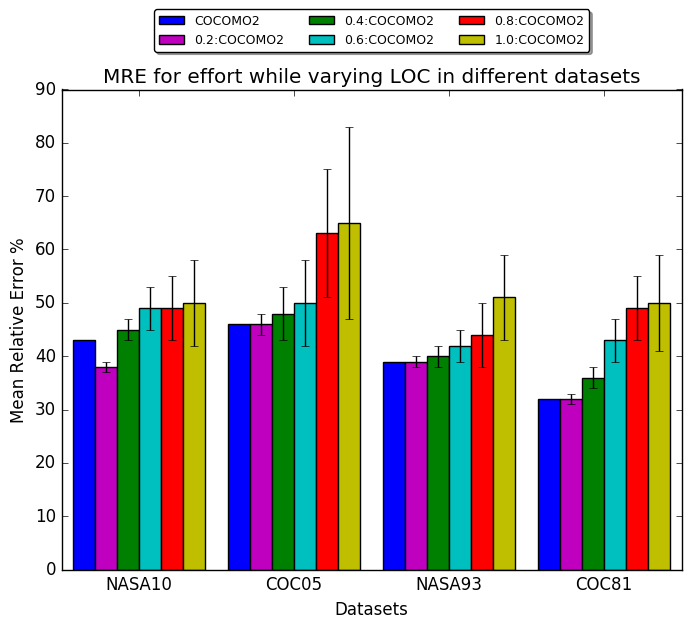
\includegraphics[scale=0.5]{Figs/mre.png}
    \caption{MRE for effor while varying LOC in different datasets.}
    \label{fig:mre_datasets}
\end{figure}

 

\section*{Acknowledgments}
The work has partially funded by a National Science Foundation CISE CCF award \#1506586.
 
\vspace*{0.5mm}
 
 
% \bibliographystyle{plain}
\bibliographystyle{elsarticle-num}
% \balance
\bibliography{refs}  

   



%   %%%%parameters for F %%%%%%
% \begin{table*}[!ht]
 
% \resizebox{\textwidth}{!}{
% % \renewcommand{\baselinestretch}{0.9}
% \scriptsize
% \centering
%   \begin{tabular}{|c |c |c |c |c |c |c |c |c |c |c |c |c |c |c |c |c |c |c |c |}
%     \hline
    
%   \begin{tabular}[c]{@{}c@{}}Learner \\ Name\end{tabular}&Parameters  & Default &antV0&antV1&antV2&camelV0&camelV1&ivy&jeditV0&jeditV1&jeditV2&log4j&lucene&poiV0&poiV1&synapse&velocity&xercesV0&xercesV1\\ 
%  \hline
% \multirow{8}{*}{\begin{tabular}[c]{@{}c@{}}Where\\based\\ Learner\end{tabular}}
% & threshold& 0.5& 0.04& 0.44& 0.44& 0.98& 0.65& 0.77& 1& 0.65& 0.98& 0.44& 0.44& 0.87& 0.04& 0.77& 0.24& 0.44& 0.77\\ \cline{2-20}
% & infoPrune& 0.33& 0.51& 0.68& 0.88& 0.47& 0.07& 0.31& 0.48& 0.68& 0.57& 0.12& 0.68& 0.01& 0.51& 0.14& 0.54& 0.68& 0.14\\ \cline{2-20}
% & min\_sample\_size& 4& 6& 4& 6& 1& 6& 8& 8& 4& 6& 7& 4& 9& 6& 2& 8& 4& 8\\ \cline{2-20}
% & min\_Size& 0.5& 0.18& 0.4& 0.56& 0.51& 0.65& 0.59& 0.97& 0.4& 0.51& 0.8& 0.4& 0.77& 0.18& 0.62& 0.46& 0.4& 0.66\\ \cline{2-20}
% & wriggle& 0.2& 0.25& 0.29& 0.76& 0.6& 0.63& 0.26& 1& 0.51& 0.17& 0.36& 0.51& 0.83& 0.25& 0.5& 0.52& 0.29& 0.26\\ \cline{2-20}
% & depthMin& 2& 3& 3& 3& 1& 5& 3& 2& 3& 5& 5& 3& 4& 3& 3& 3& 3& 3\\ \cline{2-20}
% & depthMax& 10& 16& 15& 15& 8& 19& 10& 7& 15& 5& 15& 15& 19& 16& 6& 19& 15& 10\\ \cline{2-20}
% & wherePrune& False& False& True& True& True& True& True& True& False& False& True& True& True& False& True& False& False& True\\ \cline{2-20}
% & treePrune& True& False& True& True& False& False& False& False& False& True& True& True& False& False& False& True& True& False\\ \cline{2-20}
% \hline
% \multirow{5}{*}{CART}
% & threshold& 0.5& 0.34& 0.25& 0.01& 0.01& 0.73& 0.53& 0.92& 0.8& 0.74& 0.54& 0.03& 0.91& 0.01& 0.01& 0.55& 1& 0.01\\ \cline{2-20}
% & max\_feature& None& 0.01& 0.01& 0.29& 0.01& 0.46& 0.75& 0.79& 0.74& 0.41& 0.81& 0.61& 0.72& 0.01& 0.01& 0.01& 0.25& 0.18\\ \cline{2-20}
% & min\_samples\_split& 2& 18& 20& 12& 2& 15& 11& 2& 18& 13& 9& 17& 16& 10& 4& 8& 3& 15\\ \cline{2-20}
% & min\_samples\_leaf& 1& 19& 16& 15& 17& 1& 1& 13& 10& 4& 3& 7& 5& 20& 7& 8& 1& 6\\ \cline{2-20}
% & max\_depth& None& 12& 2& 15& 1& 41& 20& 44& 15& 13& 5& 23& 14& 1& 5& 17& 47& 13\\ \cline{2-20}
% \hline
% \multirow{6}{*}{\begin{tabular}[c]{@{}c@{}}Random \\ Forests\end{tabular}} 
% & threshold& 0.5& 0.01& 0.35& 0.3& 0.01& 0.9& 0.97& 0.63& 1& 0.73& 0.68& 0.01& 1.0& 0.01& 0.07& 0.22& 1& 0.82\\ \cline{2-20}
% & max\_feature& None& 0.63& 0.17& 0.01& 0.01& 0.88& 0.74& 0.76& 0.73& 0.01& 0.03& 0.39& 0.02& 0.01& 0.56& 0.36& 0.51& 0.89\\ \cline{2-20}
% & max\_leaf\_nodes& None& 40& 33& 46& 22& 11& 16& 38& 34& 30& 31& 12& 49& 25& 47& 15& 39& 24\\ \cline{2-20}
% & min\_samples\_split& 2& 10& 16& 20& 1& 1& 1& 1& 4& 20& 19& 11& 14& 2& 17& 19& 20& 19\\ \cline{2-20}
% & min\_samples\_leaf& 1& 4& 15& 9& 13& 18& 11& 3& 16& 17& 6& 10& 7& 19& 13& 11& 2& 14\\ \cline{2-20}
% & n\_estimators& 100& 120& 73& 75& 130& 97& 144& 125& 97& 80& 111& 96& 101& 50& 67& 74& 63& 66\\ \cline{2-20}
% \hline  \end{tabular}
% }
%   \caption{Parameters tuned on different models over the objective of ``F''.}\label{tab:fselect}
% \end{table*}
 
  
% \clearpage
% \pagenumbering{roman}
% \setcounter{page}{1} 
% \section*{Reply to Reviews}

% Thank your for your comments. The typos listed by reviewers
% have been fixed and the remainder of the paper has been given
% a careful proof read.

% The reviewers raised certain issues which we respond  to as follows.

% {\em I am concerned about the reproduction of work from elsewhere. Although the relevant paper and book are cited in section 2.3 ([27, 28]) the amount of material that is reproduced is surprisingly large. I am also unsure what "presenting some new results from Rahman et al. [28]" actually means. It would obviously be wrong to present other researchers' results as if newly discovered but I doubt that this is the intention. Indeed, on checking the other paper, there is no obvious overlap. This needs to be clarified.}

% Apologies to the reviewer for our unclear text that suggests
% that this paper inappropriately copied  content from
% elsewhere. This is not the case since nearly all of this paper has not been submitted
% or published to another venue. The exception to that is:
% \bi
% \item Section 2.3 and Table1 contains 1 page of tutorial material which we have adapted from other papers.
% e.g. as the reviewer correctly points out,
% the  'Easy to use' paragraph is taken nearly verbatim from [28], as are the 'widely-used', and 'useful' paragraphs.
% \ei
% Note that apart from Section 2.3,  10 of the 11 pages of this text are   completely new.

% As to the reference to " presenting some new results from Rahman et al. [28]", that refers to one paragraph (120 words) end of section 2.3. 
% Please note that we have removed the misleading text that raised that confusion
% (start of 2.3).

% {\em I think the way that the results are presented does not do justice to the findings in the abstract (that the improvements are large, and the tuning is simple). In particular, tables 8 and 9 are not very clear; why show the naive column?}

% Thank for your that comment- we have simplified that presentation by separating the tuning \#evaluations from the runtimes-- see Table 8 and the new Table 9.

% {\em I am distracted by the frequent use of footnotes. If the material is important and worthy of mention then it should be included in the main body of the paper. However, a reference to the relevant work may be sufficient and is sometimes preferable to using a footnote.}

% Quite true- those footnotes are needlessly distracted.
% They have now been incorporated into the text.



% {\em  Eq 1 - what are d and T? - please use a where clause}



% That where clause is now added after Equation 1. That clause says

% \begin{quote} ... where  $d_i$ is the number of observed issues and $T$
% is some threshold defined by an engineering judgement; we use $T=1$.\end{quote}


\end{document}
 
\subsection{Implications}

time for an end to era of data mining in se? moving on to a new phase of learning-as-optimization

1) learning is actually an optimization tasks (e.g. see fig2 of  learners climbing the roc curve hill in http://goo.gl/x2EaAm)

2) our learners are all contorted to do some tasks X (e.g. minimize expected value of entropy), then we assess them on score Y (recall). which is nuts. maybe we should build the goal predicate into the learner (e.g http://menzies.us/pdf/10which.pdf) 

3) given 1 + 2, maybe the whole paradigm of optimizing param selection is wrong. maybe what we need is a library of bees buzzing around making random choices (e.g. about descritziation) which other bees use, plus their own random choices (e.g. max depth of tree learned from discretized data) which is used by other bees, plus their own random choices (e.g. business users reading the models).  the funky thing here is that it can take some time before some of the bees (the discretizers) get feedback from the community of people using their decision (the tree learners). 




